\documentclass[resume]{subfiles}

\begin{document}
\section{Codage de source}
Aucune connaissance de la source, son rôle est de minimiser la redondance
\paragraph{Dilemme} : Si on supprime des bits dans la source, on doit en rajouter dans le canal pour augmenter la robustesse.
\subsection{Entropie}
Symboles $\lbrace a_0, a_1, a_2, \cdots, a_{n-1}\rbrace$\\
Probabilités : $\lbrace P(a_0), P(a_1), P(a_2), \cdots, P(a_{n-1})\rbrace$
Information contenue dans un message :
$$I(a_k)=-\log_2(P(a_k))$$
Entropie de la source (moyenne du contenu d'information):
$$H=-\sum_{i=0}^{n-1}P(a_i)I(a_i)$$
\subsection{Lempel Ziv}
\begin{figure}[H]
\centering
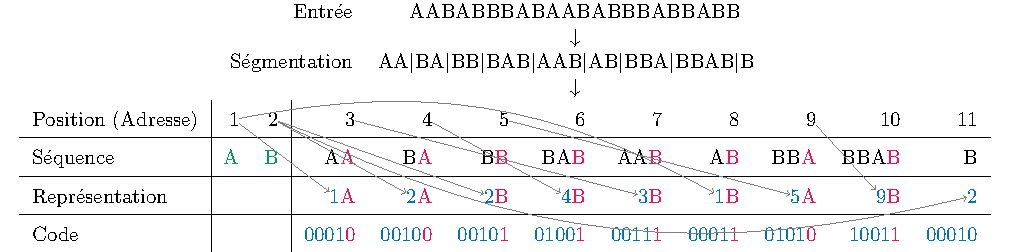
\includegraphics[width=\columnwidth]{drwg_0.pdf}
\end{figure}
\end{document}